\chapter{Domain Driven Design}
\textit{Domain Driven Design} beschreibt eine Form der Herangehensweise an die Modellierung von Software.
Dabei wird das Design der Software maßgeblich von der Fachlichkeit der Anwendungsdomäne bestimmt, indem das Domänenmodell die Grundlage für den Entwurf und die Umsetzung der Software ist.
Ein Problem stellt dabei die Komplexität dar.
Die zwei Formen der Komplexität sind die inhärente Komplexität (die Komplexität der Domäne) sowie die versehentliche Komplexität (zum Beispiel die Komplexität durch Hardware, Framework oder Infrastruktur) und ergeben zusammen die Systemkomplexität.
Dabei ist die Komplexität der Domäne fest gegeben.
Das Ziel ist das Verhindern, dass durch die technische Umsetzung die Gesamtkomplexität negativ beeinflusst wird.

Möglich wird dies durch die Reduktion des Überstzungsaufwands.
Wichtig ist dabei, das Fachgebiet mit dem Sourcecode zu vereinheitlichen.
Dazu zählt, im Sourcecode gleiche Begriffe wie in der Domäne zu verwenden und eine klare Modellierung der Fachlichkeit.

Eine weitere Möglichkeit zur Vermeidung der negativen Beeinflussung der Gesamtkomplexität, ist die Beschreibung von nützlichen Methoden und Muster.
Es gibt diesbezüglich zwei Richtungen: das strategische \ac{DDD}, dass auf die Analyse, die Dokumentation sowie die Abgrenzung der Domäne abzielt und das taktische \ac{DDD}, dass die Erkenntnisse in Sourcecode umsetzt.

In Bezug auf den Softwareentwurf ist die Analyse der \textit{Ubiquitous Language} relevant.
Ubiquitous Language bezeichnet die von Domänenexperten und Entwicklern gemeinsam verwendete Sprache.
Schließlich ist die jeweilige Fachsprache des einen nur schwer für die andere Partei zu verstehen.
Somit würde sich der Sourcecode von der Sprache der Domäne entfernen und daraus resultiert eine höhere Komplexität und ein schwereres Verständnis der Implementierung.
Die entstehende Kluft soll reduziert werden, indem alle relevanten Konzepte, Prozesse und Regeln der Domäne erklärt sind.
Zudem werden Zusammenhänge verdeutlicht.
Mehrdeutigkeiten und Unklarheiten sollen durch die Definition der \textit{Ubiquitous Language} beseitigt werden und die Domänensprache sollte dabei im Softwaredesign, der Dokumentation und der Bedienungsoberfläche beibehalten werden.
Zu beachten ist hierbei, dass sich allerdings auf den Kern des Projekts fokusiert wird.

Darüber hinaus werden in \ac{DDD} die Grundbausteine eines Modells definiert.
Innerhalb dieses Softwareentwurfs werden die Bausteine 
\begin{itemize}
    \item \textit{Repositories}, 
    \item \textit{Aggregates},
    \item \textit{Entities} und
    \item \textit{Value Objects}
\end{itemize}
betrachtet.

\textit{Repositories} dienen als sogenannte \glqq Voratsschränke\grqq{} des Systems und bieten den Zugriff auf den persistenten Speicher.
Dadurch wird der Code der Domäne von den technischen Details der Speicherung getrennt.
Ähnlichkeiten sind hierbei zur \textit{Clean Architecture} zu erkennen.

\textit{Entities} bezeichnen Objekte, die entsprechend ihrer Identität modelliert werden.
Identitäten gibt es in mindestens drei Formen: der Kombination von Eigenschaften, einem Surrogatschlüssel oder der natürliche Schlüssel.
Die Werte der \textit{Entities} sind veränderlich.

\textit{Value Objects} sind einfache Objekte ohne eigene Identität.
Die Werte der \textit{Value Objects} sind unveränderlich und \textit{Value Objects} sind gleich, wenn deren Werte gleich sind.

\textit{Aggregates} gruppieren \textit{Entities} sowie \textit{Value Objects} zu gemeinsam verwalteten Einheiten.
Bei \textit{Aggregates} übernimmt ein \textit{Aggregate Root} die Zugriffe von außen.


\section{Analyse und Begründung der \textit{Ubiquitous Language}}
Zum Verständnis der Software wurde eine \text{Ubiquitous Language} festgelegt, indem sich an der Domäne der Anwendung orientiert wurde.
Die Domäne bezieht sich auf das Verwalten von Konsumgütern.
Die Konsumgütern können in einem Kühlschrank oder einem Regal aufbewahrt werden.
Konsumgüter haben eine Gewichtseinheit.
Eine Form der Konsumgüter, die derzeit verwaltet werden soll, sind Lebensmittel.
Ein Lebensmittel hat ein Mindesthaltbarkeitsdatum.

\todo[]{Darstellung Prozesse Einlagern, Updaten, Auslagern}

Diese Informationen über die Domäne wurden in die \textit{Ubiquitous Language} berücksichtigt.
Die Abbildung \ref{fig:wordcloud} des geschriebenen Codes in einer Wordcloud verdeutlicht die Umsetzung der \textit{Ubiquitous Language}.

\begin{figure}[H]
	\centering
	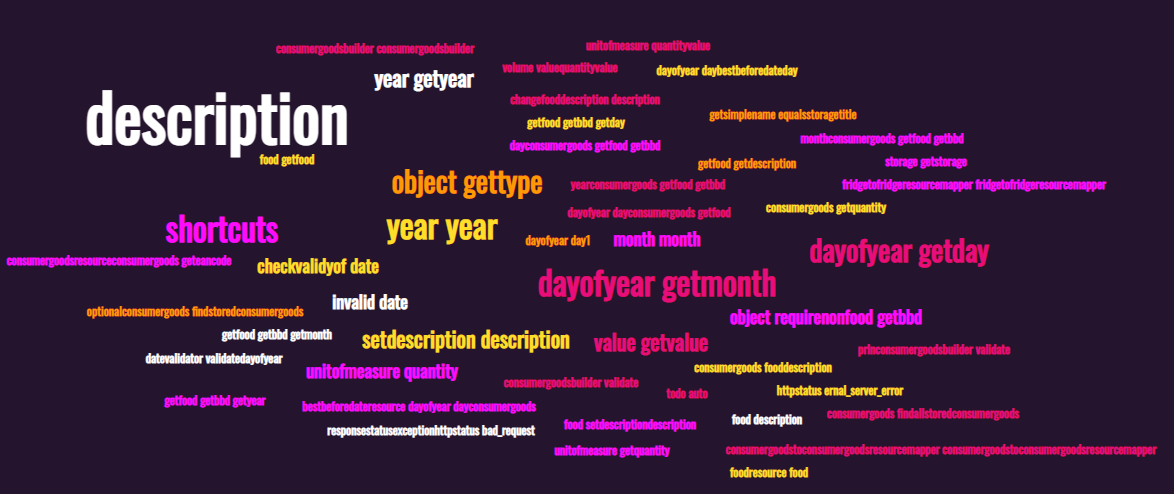
\includegraphics[width=1.0\textwidth]{Bilder/wordcloud.PNG}
	\caption[Wordcloud in Bezug zur Verdeutlichung der Umsetzung Ubiquitous Language.]{Die Wordcloud visualisiert die verwendeten Bezeichnungen im Programentwurf in Bezug auf die \textit{Ubiquitous Language}. Die Wordcloud verdeutlicht, dass die \textit{Ubiquitous Language} umgesetzt wurde, indem statt rein technischen Begriffen hauptsächlich Bezeichnungen mit Domänenbezug benannt wurde.}
	\label{fig:wordcloud}
\end{figure}

Eine Umsetzung der \textit{Ubiquitous Language} ist die Benennung der Klassen.
Die Klasse \href{}{\code{ConsumerGoods}} repräsentiert gleichnamige Konsumgüter.
%Dazu zählt eine Assoziation auf die Klasse vom Typ \textit{StorableGoods}, wozu auch die Klasse \textit{Food} zählt, die Lebensmittel repräsentieren.
Dazu zählt eine Assoziation auf die Klasse \href{}{\code{Food}}, die Lebensmittel repräsentieren.
Lebensmittel haben ein Mindesthaltbarkeitsdatum, dass in der assoziierten Klasse \href{}{\code{BestBeforeDate}} verwaltet wird.
Das Mindesthaltbarkeitsdatum wird durch die assoziierten Klassen \href{}{\code{DateOfYear}} und \href{}{\code{Year}} repräsentiert.
Ein \textit{DateOfYear} setzt sich aus den Klassen \href{}{\code{Day}} und \href{}{\code{Month}} zusammen, die entsprechend das Datum des Tages und das Datum des Monats repräsentieren.
Die Entscheidung für die Repräsentation eines Tages des Jahres durch die Klasse \href{}{\code{}}\code{DateOfYear} ist, dass das MHD oftmals innerhalb eines Jahres liegt und bei der Validierung des Datums nur im Monat Februar das Jahr relevant ist.
Die Klasse \href{}{\code{DateValidator}} übernimmt die entsprechende Aufgabe der Datumsvalidierung.
Hinzu kommen die Klassen \href{}{\code{DayValidator}}, \href{}{\code{MonthValidator}} und \href{}{\code{YearValidator}}.
Diese Klassen dienen entsprechend ihrer Bezeichnung der Validierung eines Wertes für einen Tag, Monat oder eine Jahreszahl.
Die Validierung beschränkt sich insofern auf die Domäne, dass bei sich bei den gültigen Werten an den gültigen Werten für ein Datum in Deutschland orientiert wird.
Daneben haben Konsumgüter eine Menge, die durch die Assoziation auf die Klasse vom Typ \href{}{\code{}}\textit{UnitOfMeasure} repräsentiert wird.
Als konkrete Maßeinheit können Gewicht, Volumen oder Stückzahl gewählt werden und werden durch die gleichnamigen Klassen \href{}{\code{}}\textit{Weight}, \href{}{\code{}}\textit{Volume} und \href{}{\code{}}\textit{Quantity} repräsentiert.
Neben der Maßeinheit dient die Klasse \href{}{\code{Value}} zur Repräsentation der quantitaven Menge.
Die Klasse \href{}{\code{ValueValidator}} übernimmt die in Bezug auf die Domäne bezogene Überprüfung eines gültigen Werts, der später durch ein Objekt der Klasse \href{}{\code{Value}}.
Bezogen auf die Regeln innerhalb der Domäne darf der Wert nicht negativ sein.

Ein Konsumgut hat zudem einen Lagerort, der durch die Assoziation zu einer Klasse des Typs \textit{Storage} repräsentiert wird.
Als mögliche Typen für Lagerorte kommen in der Domäne Kühlschränke oder Lebensmittelregale in Frage, die durch die gleichnamigen Klassen \textit{Fridge} und \textit{FoodShelf} dargestellt sind.

Die Interfaces \href{}{\code{ConsumerGoodsRepository}}, \href{}{\code{FridgeRepository}} sowie \href{}{\code{FoodShelfRepository}} dienen zur Implementierung von, ebenfalls in \ac{DDD} definierten, Repositories in Bezug auf die Klassen \href{}{\code{}}\textit{ConsumerGoods}, \href{}{\code{}}\textit{Fridge} und \href{}{\code{}}\textit{FoodShelf}.
Repositories werden im Abschnitt \ref{domaindrivendesign>repositories} analyisiert.
Die Bezeichnung \textit{-Repository} ist in diesem Fall möglich, da es sich hierbei um das \ac{DDD}-Modell \textit{Repository} handelt und dieses somit direkt ersichtlich wird.

Die Klassen \href{}{\code{ConsumerGoodsManager}} und \href{}{\code{StorageManager}} repräsentieren die Umsetzung der Busines-Logik und diese entspricht dem Managen von Konsumgütern und Lagerorten. 

\href{}{\code{ConsumerGoodsToConsumerGoodsResourceMapper}}, \href{}{\code{StorageToStorageResourceMapper}} und die Klassen \href{}{\code{ConsumerGoodsResource}} und \textit{StorageResource} sind mit dem Zusatz -Resource beschrieben, da es sich hierbei um Resourcen der Domänenklassen handelt, die zur Verarbeitung mit den äußeren Schnittstellen, wie zum Beispiel der \ac{GUI}, verwendet werden.

Die Klassen \href{}{\code{ConsumerGoodsGuiInterface}} sowie \href{}{\code{StorageInteractorGuiInterface}} sind aufgrund ihrer Funktion als Schnittstelle für die Informationsübertragung an die GUI.

\href{}{\code{ConsumerGoodsBridge}}, \href{}{\code{FoodShelfRepositoryBridge}} und \href{}{\code{FridgeRepositoryBridge}} erfüllen die Funktion des \textit{Bridge}-Entwurfsmusters in Bezug auf die Repositories der Domänen \textit{ConsumerGoods}, \textit{Fridge} und \textit{FoodShelf} und haben dementsprechend die Bezeichnung.
Bei den Interfaces \href{}{\code{PersistenceConsumerGoodsRepository}}, \href{}{\code{PersistenceFridgeRepository}} und \href{}{\code{PersistenceFoodShelfRepository}} wurde die entsprechende Bezeichnung gewählt, da es sich hierbei um Klassen handelt, die entsprechend dem \ac{DDD} die Funktion des \textit{Repositories} umsetzen.
Die Bezeichnung \textit{Persistence-} wurde gewählt, da die Interfaces zur Implementierung der Persistierung dienen.

\subsection*{Umsetzung der Ubiquitos Language auf der grafischen Oberfläche}
In der GUI wurde ebenfalls die \textit{Ubiquitos Language} angewandt.
Beim Anlegen eines Konsumguts wurde die Bezeichnung der Domäne, das Einlagern, sowie beim Löschen, das Auslagern, verwendet und in der Oberfläche beschriftet.

\begin{figure}[H]
	\centering
	
\includegraphics[width=0.3\textwidth]{Bilder/gui/Ubiquitous Language/store-text.PNG}
	\caption[Überschrift Eingabemaske zum Einlagern eines Konsumguts.]{Anstatt der technischen Bezeichnung, dem Speichern eines Konsumguts, wird die domänenspezifische Bezeichnung des Einlagerns verwendet.}
	\label{fig:gui-titel-einlagern}
\end{figure}

\begin{figure}[H]
	\centering
	
\includegraphics[width=0.7\textwidth]{Bilder/gui/Ubiquitous Language/outsource-text.PNG}
	\caption[Bezeichnung eines Auslagerungsvorgangs.]{Beim Auslagern eines Konsumguts erhält der Anwender eine domänenbezogene Rückmeldung und wird nicht gefragt, ob er den technischen Vorgang, das Löschen des Konsumguts, durchführen möchte.}
	\label{fig:gui-titel-auslagern}
\end{figure}

Auch die Identifikationsnummer wurde anstatt \textit{id} der Domäne angepasst und \textit{EAN} bezeichnet. 

\begin{figure}[H]
	\centering
	
\includegraphics[width=0.3\textwidth]{Bilder/gui/Ubiquitous Language/ean.PNG}
	\caption[Darstellung EAN-Code.]{Der natürliche Schlüssel der Domäne wird zur eindeutigen Identifikation genutzt und dargestellt.}
	\label{fig:gui-darstellung-ean}
\end{figure}

Ebenfalls wurden Buttons anstatt den technischen Eigenschaften Einfügen und Löschen passend zur Domäne beschriftet.

\begin{figure}[H]
	\centering
	
\includegraphics[width=0.3\textwidth]{Bilder/gui/Ubiquitous Language/Store new consumer good.PNG}
	\caption[Button zum Öffnen der Eingabemaske zum Einlagern eines Konsumguts.]{.}
	\label{fig:gui-button-eingabemaske-einlagern}
\end{figure}

\begin{figure}[H]
	\centering
	
\includegraphics[width=0.5\textwidth]{Bilder/gui/Ubiquitous Language/store-buttons.PNG}
	\caption[Buttons zum Bestätigen des Einlagerns eines Konsumguts.]{Die Buttons zum technischen Speichern und Abbrechen sind ebenfalls entsprechend des Domänenkontext beschrieben.}
	\label{fig:gui-button-einlagern}
\end{figure}

\begin{figure}[H]
	\centering
	
\includegraphics[width=0.5\textwidth]{Bilder/gui/Ubiquitous Language/edit-buttons.PNG}
	\caption[Buttons zum Bestätigen von Änderungen der Attribute eines Konsumguts.]{Die Buttons zum Bestätigen von Änderungen an einem Konsumgut sind ebenfalls entsprechend des Domänenkontext beschrieben.}
	\label{fig:gui-button-aendern}
\end{figure}

\begin{figure}[H]
	\centering
	
\includegraphics[width=0.5\textwidth]{Bilder/gui/Ubiquitous Language/outsource-buttons.PNG}
	\caption[Buttons zum Bestätigen des Auslagern eines Konsumguts.]{Die Buttons zum technischen Löschen sind ebenfalls entsprechend des Domänenkontext beschrieben.}
	\label{fig:gui-button-auslagern}
\end{figure}

Das Anwenden der \textit{Ubiquitos Language} auf der grafischen Oberfläche hat den allgemeinen Vorteil, dass Abläufe und Funktionen für den Anwender, der mit der Domäne vertraut ist, bei der Anwendung der Software verständlicher sind und Missverständnisse reduziert werden.

Grundsätzlich handelt es sich bei diesem Softwareentwurf um eine \ac{CRUD}-Anwendung.
Die Anwendung dient dem Verwalten von Konsumgütern an Lagerorten.
Die Komplexität ist dabei relativ gering, weshalb man solche Anwendungen als \textit{Smart UI}-Anwendungen bezeichnet.
Dementsprechend wurden nur eine geringe Anzahl an \ac{DDD}-Modelle angewandt, da das Einfügen zusätzlicher Modelle die Komplexität der Anwendung künstlich steigern würde.

Im Folgenden werden die angewandten \ac{DDD}-Modelle \textit{Entities}, \textit{Value Objects}, \textit{Aggregates} und \textit{Repositories} aufgezeigt und in ihrer Funktion innerhalb des Softwareentwurfs analysiert.

\section{Analyse angewandter Value Objects}
\label{domaindrivendesign>valueobjects}
Innerhalb des Softwareentwurfs werden \textit{Value Objects} zur Repräsentation eines Wertes verwendet.
Dazu zählen die Klassen \href{}{\code{Day}}, \href{}{\code{Month}}, \href{}{\code{Year}} sowie \href{}{\code{Value}}.
Die Klassen \href{}{\code{}}\textit{Day}, \href{}{\code{}}\textit{Month} und \href{}{\code{}}\textit{Year} dienen dabei dem Speichern des gleichnamigen Teils des Datums.
Die Klasse \href{}{\code{}}\textit{Value} speichert den Wert der dazugehörigen Einheit innerhalb der Klassen \href{}{\code{}}\textit{Volume}, \href{}{\code{}}\textit{Quantity} oder \href{}{\code{}}\textit{Weight}.
Die Werte sind insofern immutable, dass eine Zuweisung des Werts, neben der Initialisierung durch den Konstruktor, nicht möglich ist.
Die Variablen innerhalb der Klassen zum Speichern der Methoden sind daher als \textit{final} gekennzeichnet.
Die Klassen enthalten zudem keine \textit{setter}-Methode.
Darüber hinaus enthalten die Klassen ausschließlich Methoden zur Rückgabe des Werts.
Der Wert wird dabei als unveränderliche Objekte zurückgegeben, um ein Verändern des Werts zu unterbinden.
Die Klassen selbst sind ebenfalls \textit{final} deklariert, um eine Vererbung auszuschließen.
Die Objekte der Klasse dienen schließlich ausschließlich der Werterepräsentation und ein Manipulieren des Wertes, auch durch Subklassen, ist auszuschließen.
\todo{Bei allen Ref und Darstellung der Anpassung der hashCode()- und equals()-Methode}
\todo[]{Ref zu Day, final und immutable (kein set außer Konstruktor) zeigen}
\todo[]{Ref zu Month, final und immutable (kein set außer Konstruktor) zeigen}
\todo[]{Ref zu Year, final und immutable (kein set außer Konstruktor) zeigen}
\todo[]{Ref zu Value, final und immutable (kein set außer Konstruktor) zeigen}
\todo[]{Felder sind blank final!}
\todo[]{Klasse ist final definiert}
\todo[]{equals und getHash anpassen}

\todo[]{gemacht, weil Fehler durch Manipulation reduziert werden sollen und Objekte eine klare Zuweisung haben sollen.}

Darüber hinaus lassen sich in diesem Softwareentwurf weitere \textit{Value Objects} erkennen, die sich aus den grundlegenden \textit{Value Objects} zusammensetzen.
Eines stellt die Klasse \href{}{\code{}}\textit{DayOfYear} dar.
Die Klasse dient der Verwaltung der \textit{Value Objects} \href{}{\code{}}\textit{Day} sowie \href{}{\code{}}\textit{Month} und repräsentiert somit den Tag eines Jahres.
Auch in diesem Fall zeichnet sich die Klasse \href{}{\code{}}\textit{DayOfYear} als \textit{Value Object} aus, da es den reinen und unveränderlichen Werten eine Semantik in der Domäne gibt und keine Identität oder Lebenszyklus aufweist.
Ein weiteres \textit{Value Object} ist die Klasse \href{}{\code{BestBeforeDate}}.
Die Klasse dient lediglich der Repräsentation eines Datums, in Bezug zur Domäne dem Mindesthaltbarkeitsdatums eines Produkts, und ist somit eine Möglichkeit, dem reinen Datum als Wert eine Semantik in der Domäne zu geben.

\todo[]{gemacht, weil übersichtlicher und lesbarer}
%Die Klasse \textit{Food} bildet als Zusammenfassung des \textit{Value Objects} \textit{BestBeforeDate} sowie der Implementierung des Interfaces \textit{UnitOfMeasure} ein weiteres \textit{Value Object}.
%Gewicht ist theoretisch änderbar?

\section{Analyse angewandter Entities}
\label{domaindrivendesign>entities}
Bei Befassung der Domäne, in der sich der Softwareentwurf befindet, fallen die grundlegenden Elemente der Domäne \href{}{\code{ConsumerGoods}}, \href{}{\code{Fridge}} sowie \href{}{\code{FoodShelf}} auf.
Es handelt sich bei diesen Klassen entsprechend \ac{DDD} um Entitäten.
Die Klasse \href{}{\code{}}\code{ConsumerGoods} repräsentiert einen Gegenstand der Domäne, ein Konsumgut.
Die Klassen \href{}{\code{}}\code{Fridge} und \href{}{\code{}}\code{FoodShelf} repräsentieren ebenfalls Gegenstände der Domäne, nämlich einen Kühlschrank und ein Lebensmittelregal.
Eine Eigenschaft von Entitäten ist das Besitzen einer Identität in Form einer Kombination von Eigenschaften oder eines Surrogat- beziehungsweise natürlichen Schlüssels.
Ein Konsumgut weist die Eigenschaft auf, dass es in der Domäne einen natürlichen Schlüssel hat.
Jedes Produkt, das käuflich im Handel erwerblich ist, hat einen \ac{EAN}.
Dementsprechend hat hat die Klasse \href{}{\code{}}\code{ConsumerGoods} den natürlichen Schlüssel \href{}{\code{}}\ac{EAN} zur eindeutigen Identifikation implementiert.
Die \ac{EAN} bezeichnet die Nummer unter dem Barcode und dient als eindeutige Produktidentifizierungsnummer.
Dabei ist zu beachten, dass die Codezuweisung fremdbestimmt ist und somit auch keine Garantie auf Duplikatfreiheit außerhalb des Kontextes gegeben werden kann.
Zudem können Produkte, die keinen \ac{EAN} haben, zum aktuellen Stand nicht in der Software verwaltet werden, da zunächst ausschließlich im Handel erwerbliche Konsumgüter verwaltet werden.
Bei der \textit{Entity} \href{}{\code{}}\code{Fridge} ist jedoch kein eindeutiger Schlüssel in der Domäne enthalten, weshalb ein Surrogatschlüssel angewandt wird.
Die Klasse \href{}{\code{}}\code{Fridge} hat hierzu eine Variable \href{}{\code{id}}, deren Wert automatisch systemseitig zur Laufzeit generiert wird.
Der Vorteil ist, dass der Schlüssel jederzeit generierbar ist, jedoch keinen Bezug zur Domäne hat.
Bei der \textit{Entity} \href{}{\code{}}\code{FoodShelf} ist ebenfalls kein eindeutiger Schlüssel in der Domäne enthalten, weshalb auch ein Surrogatschlüssel angewandt wird.
Die Generierung läuft entsprechend gleich zu der in der Klasse \href{}{\code{}}\code{Fridge} ab.

\todo[]{gemacht, weil Abbildungen aus der Realität}

\section{Analyse angewandter Aggregates}
\label{domaindrivendesign>aggregates}
In diesem Softwareentwurf dienen die Klassen \href{}{\code{ConsumerGoods}}, \href{}{\code{Fridge}} und \href{}{\code{FoodShelf}} als \textit{Aggregates}.
Bei Analyse des größten \textit{Aggregates} innerhalb des Softwareentwurfs ist zu erkennen, dass neben der \textit{Entity} \href{}{\code{}}\textit{ConsumerGoods} auch eine Implementierung des Interfaces \href{}{\code{}}\textit{StorableGoods}, was in dem aktuellen Stand nur auf die Klasse \href{}{\code{}}\textit{Food} zutrifft, zu diesem \textit{Aggregate} zählen. 
Zudem zählen die \textit{Value Objects} \textit{BestBeforeDate} als auch eine Implementierung des Interfaces \textit{UnitOfMeasure} hinzu.

\todo[]{Visualisierung des Aggregates}

Bei Betrachtung der Visualisierung des \textit{Aggregates} ist zu erkennen, dass ein Zugriff auf die Objekte innerhalb des \textit{Aggregates} über das Objekt der Klasse \href{}{\code{}}\textit{ConsumerGoods} erfolgen.
Es handelt sich somit beim Objekt der Klasse \href{}{\code{}}\textit{ConsumerGoods} um ein \textit{Aggregate Root}.
Direkte Referenzen auf Elemente innerhalb des \textit{Aggregates} sind dabei nicht erlaubt.
Eine Betrachtung des UML-Diagramms im Kapitel \href{}{\code{}}\todo[]{ref zu UML} zeigt jedoch, dass solch eine direkte Referenz nicht vorliegt und der Zugriff ausschließlich über den \textit{Aggregate Root} funktioniert.
\todo[]{Aktuell durch Resource verletzt, entweder ändern und erläutern oder Verletzung erläutern}

Ein Objekt der Klasse \href{}{\code{}}\textit{ConsumerGoods} kann somit den gesammten Zugriff auf das \textit{Aggregate} kontrollieren und die Einhaltung der Domänenregeln gewährleisten.
Ein Beispiel ist in diesem Fall die Validierung des eingegebenen Mindesthaltbarkeitsdatums durch die Klasse \href{}{\code{}}\textit{DateValidator}.
Durch das \textit{Aggregate Root} kann die Einhaltung der Domänenregel, nämlich der Angabe eines gültigen Datums, validiert und gewährleistet werden.

Das \textit{Aggregate Root} \textit{ConsumerGoods} ist über die ID \href{}{\code{}}\textit{eanCode} eindeutig identifizierbar.
Ein Verlust dieser ID zur Laufzeit führt dazu, dass neben dem Objekt der Klasse \href{}{\code{}}\textit{ConsumerGoods} das gesammte \textit{Aggregate} und somit das dazugehörige Objekt der Klasse \href{}{\code{}}\textit{Food}, \href{}{\code{}}\textit{BestBeforeDate} als auch das Objekt der Implementierung des Interfaces \textit{UnitOfMeasure} nicht mehr erreichbar.
Die Herausgabe von Referenzen auf innere Objekte werden zur Gewährleistung des den Domänenregeln entsprechenden Zustands Kopien oder Immutable-Dekorierer ausgegeben, wie \href{}{\code{}}in diesem Beispiel zu erkennen \todo{Ref einfügen}.

Des Weiteren werden bei \ac{CRUD}-Anwendungen auf einzelne Objekte des \textit{Aggregates} das gesammte \textit{Aggregate} geladen und entsprechend gespeichert, wie in \href{}{\code{ConsumerGoodsApplicationService}} zu erkennen.
Das Ziel ist die Minimierung des Risikos auftretender Bugs durch ungültige Zustände aufgrund teilweiser Änderungen sowie die Einhaltung der Domänenregeln durch das \textit{Aggregate Root}, über das die \ac{CRUD}-Anwendungen ausgeführt und an den entsprechenden internen Objekten angewandt werden.

Der Vorteil bei der Bildung dieses \textit{Aggregates} ist, dass durch den zentralen Zugriff über das \textit{Aggregate Root} die Domänenregeln eingehalten werden können.
Des Weiteren wird durch die Einteilung in einzelne \textit{Aggregates} Transaktionsgrenzen gebildet und übergreifende Objektbeziehungen ebenfalls durch den zentralen Zugriff entkoppelt.

Bei den \textit{Aggregates} \href{}{\code{}}\textit{Fridge} und \href{}{\code{}}\textit{FoodShelf} handelt es sich um Implementierung des Interfaces \href{}{\code{}}\textit{Storage}.
Die \textit{Aggregates} haben zum aktuellen Stand keine Referenzen auf weitere Klassen und sind somit zugleich \textit{Aggregate Root}, auch in Hinblick auf ihre Funktion mit möglichen Erweiterungen.

\todo[]{gemacht, weil dadurch klare Abgrenzungen und eine bessere Verwaltbarkeit vorliegt, Bearbeiten und Verändern von Attributen oder Teilen des Aggregates und daraus resultierende Fehler somit minimiert}

\section{Analyse angewandter Repositories}
\label{domaindrivendesign>repositories}
Innerhalb dieses Softwareentwurfs übernehmen die Interfaces \href{}{\code{ConsumerGoodsRepository}}, \href{}{\code{FridgeRepository}} sowie \href{}{\code{FoodShelfRepository}} die Funktion des \textit{Repositories} als \ac{DDD}-Modell.
Dabei ist laut \ac{DDD} vorgesehen, dass \textit{Repositories} direkt mit \textit{Aggregates} zusammenarbeiten und somit für jedes der im Softwareentwurf definierten \textit{Aggregates} \href{}{\code{ConsumerGoods}}, \href{}{\code{Fridge}} als auch \href{}{\code{FoodShelf}} ein \textit{Repository}-Modell vorhanden ist.

Die Bezeichnung der Methoden ist ebenfalls an die Domäne angepasst, wie anhand eines Beispiels an der Klasse \href{}{\code{}}\textit{ConsumerGoodsRepository} zu sehen ist.

Die konkrete Implementierung der Persistierung findet in den jeweils entsprechenden Klassen \href{}{\code{ConsumerGoodsRepositoryBridge}}, \href{}{\code{FridgeRepositoryBridge}} sowie \href{}{\code{FoodShelfRepositoryBridge}} statt.
Dies ist sowohl für das \ac{DDD}-Modell \textit{Repository} als auch entsprechend der \textit{Clean Architecture} entsprechend vorgesehen, dass die Implementierung außerhalb stattfindet. 
Schließlich zählt die Definition des \textit{Repository} zum \textit{Domain Code}, die konkrete Umsetzung ist jedoch domänenunabhängig oder auch \textit{Pure Fabrication} genannt.

\todo[]{gemacht, weil zentrale Verwaltungsmöglichkeit}
